\documentclass[12pt,a4paper]{article}
\usepackage[utf8]{inputenc}
\usepackage[french]{babel}
\usepackage[T1]{fontenc}
\usepackage{amsmath}
\usepackage{amsfonts}
\usepackage{amssymb}
%Appeldupackagepythontex
\usepackage{pythontex}
%

\usepackage{graphicx}

\title{Test PythonTex}
\author{Romain}



\begin{document}
%%%%%%%%%%%%%%%%%%%%%%%%%%%%%%%%%%%%%%%%%%%%%%%%%%%%%%%%%%%%%%%%%%%%%%%%%%%%%%%%%%%%%%%%%%%
\maketitle

\begin{pycode}
from sympy import *
x=symbols('x')
f = (x**5)*ln(x)
g = Integral(f,x)
\end{pycode}
%
$\py{latex(g)} = \py{latex(g.doit())}$
%
\begin{pyverbatim}
import math

def racine(a):
    return math.sqrt(a)

print(racine(9))
\end{pyverbatim}


\bigskip

Résultat : 

\begin{pycode}
import math

def racine(a):
    return math.sqrt(a)

print(racine(9))
\end{pycode}
%
\begin{pyconsole}
var = 1 + 1
var
\end{pyconsole}



%
\begin{pycode}
import numpy as np
from pylab import *
import matplotlib.pyplot as plt


def f(t):
	return cos(3*t)
	
t = np.linspace(0,5,500)

y = f(t)

plt.clf()
plt.figure(figsize=(5, 3))
plt.plot(t,y)

plt.savefig("myplot.pdf", bbox_inches="tight")
\end{pycode}
%



\begin{center}
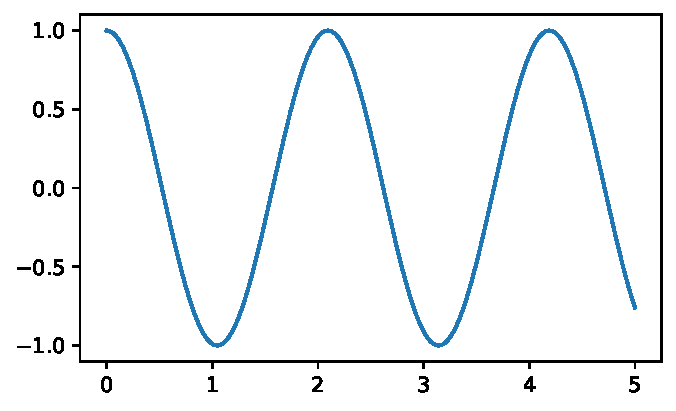
\includegraphics[width = 0.85\textwidth]{myplot.pdf}
\end{center}

%t = linspace(0,5,500)
%y = f(t)

%clf()
%figure(figsize(5,3))
%rc("text", usetex=True)

%plot(t, y)
%title("Décroissance exponentielle amortie")
%text(3, 0.15, r"$y=\cos(2\pi t)e^(-t)$")
%xlabel("time (s)")

%savefig("myplot.pdf", bbox_inches = "tight")

%print(r"\begin{center}")
%print(r"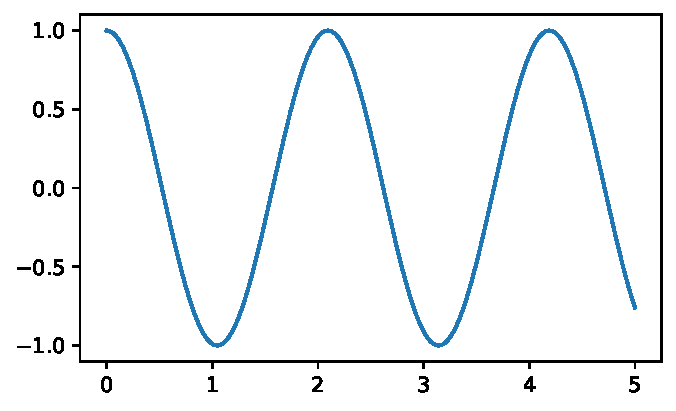
\includegraphics[width=0.85\textwidth]{myplot.pdf}")
%print(r"\end{center}")

%%%%%%%%%%%%%%%%%%%%%%%%%%%%%%%%%%%%%%%%%%%%%%%%%%%%%%%%%%%%%%%%%%%%%%%%%%%%%%%%%%%%%%%%%%%
\end{document}

